\documentclass{article}

\usepackage{geometry}
\geometry{
	a4paper,
	total={170mm,257mm},
	left=20mm,
	top=20mm,
}

\usepackage{graphicx}
\usepackage{subfig}
\usepackage{amsmath}
\usepackage{url}
\usepackage{enumitem}
\usepackage{footnote}
\makesavenoteenv{table}
\makesavenoteenv{tabular}
\usepackage{multirow}
\usepackage{listings}


\begin{document}

\section{Reset the numbering of subfigure in LaTeX}
\begin{figure}[h!]
	\centering
	\subfloat[Kitten 1]{
		\centering
		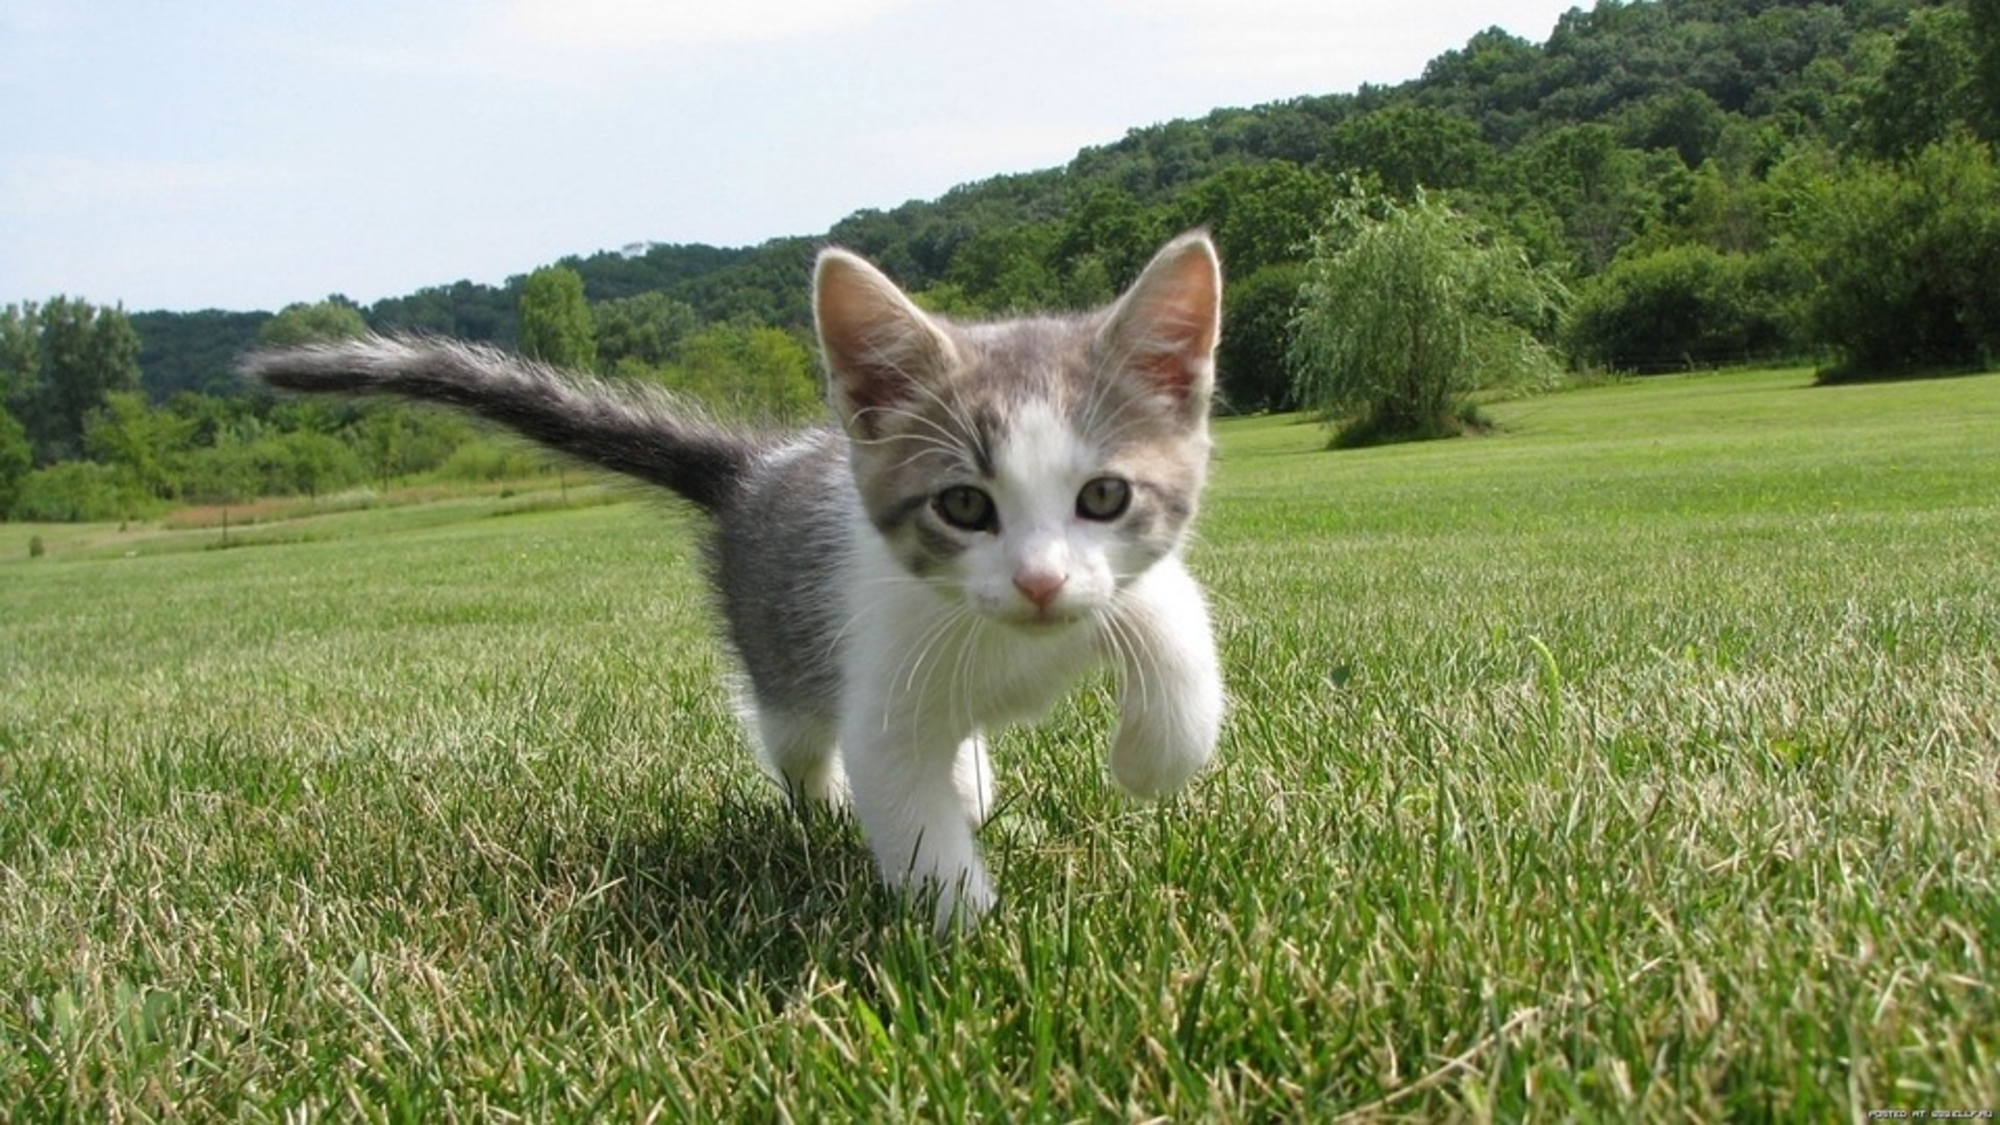
\includegraphics[width=.45\textwidth]{imgs/kitten_0.pdf}
	}
	\setcounter{subfigure}{0}
	\subfloat[Kitten 2]{
		\centering
		\includegraphics[width=.45\textwidth]{imgs/kitten_1.pdf}
	}
	\caption{
		Kittens: Reset the numbering in between the figures, 
		so the numbers are both (a).
	}
	\label{fig:fig1}
\end{figure}


\section{Math mode}

\subsection{Arrow with text}
\[kitten \xrightarrow{is} cute\]

\subsection{Norm}
\[\lVert A \rVert\]


\section{Tables}
\begin{itemize}
	\item Use url environment in caption of table
	\item Footnote in the table and tabular environment
	\item Partial line in a table
	\item Rotate text on multirow environment
\end{itemize}

\begin{table}[h!]
	\centering
	\caption{hoge \protect\url{https://github.com/Taka-Coma/LaTeXMemo} fuga}
	\begin{tabular}{|c|c|}
		\hline
		\multirow{2}{*}{\rotatebox[origin=c]{90}{hoge}} & huga \\
		\cline{2-2}
		 & fuga\footnote{fugafuga} \\
		\hline
	\end{tabular}
	\label{tab:table1}
\end{table}



\section{Shorten left margin of itemize/enumerate/description}

\paragraph{Normal}

\begin{itemize}
	\item hoge
	\item fuga
\end{itemize}

\paragraph{Shortened}

\begin{itemize}[leftmargin=*]
	\item hoge
	\item fuga
\end{itemize}


\section{Hyphen in math}

\paragraph{Hyphen as minus (fail)}

\[ TF-IDF(t, d) = df(t, d) \cdot idf(t) \]

\paragraph{Hyphen in math (success)}

\[ TF\mbox{-}IDF(t, d) = df(t, d) \cdot idf(t) \]


\section{Combination notation}

\[ N\choose{i} \]


\section{Circled number}

\[\textcircled{\scriptsize 1}\]


\section{Change the numbering rules of lstlisting}

\begin{lstlisting}[
	captionpos=b,
	caption=caption
]
test without section number
\end{lstlisting}

\renewcommand{\thelstlisting}{\thesection.\arabic{lstlisting}}

\begin{lstlisting}[
	captionpos=b,
	caption=caption
]
test with section number
\end{lstlisting}


\end{document}
